%%%%%%%%%%%%%%%%%%%%%%%%%%%%%%%%%%%%%%%%%%%%%%%%%%%%%%%%
%                       Assignment 2                   %
%                                                      %
% Author: Michael P. J. Camilleri					   %
%                                                      %
% Based on the Cleese Assignment Template for Students %
% from http://www.LaTeXTemplates.com.				   %
%                                                      %
% Original Author: Vel (vel@LaTeXTemplates.com)		   %
%													   %
% License:											   %
% CC BY-NC-SA 3.0 									   %
% (http://creativecommons.org/licenses/by-nc-sa/3.0/)  %
% 													   %
%%%%%%%%%%%%%%%%%%%%%%%%%%%%%%%%%%%%%%%%%%%%%%%%%%%%%%%%

%--------------------------------------------------------
%   IMPORTANT: Do not touch anything in this part
\documentclass[12pt]{article}
%%%%%%%%%%%%%%%%%%%%%%%%%%%%%%%%%%%%%%%%%
% Cleese Assignment
% Structure Specification File
% Version 1.0 (27/5/2018)
%
% This template originates from:
% http://www.LaTeXTemplates.com
%
% Author:
% Vel (vel@LaTeXTemplates.com)
%
% License:
% CC BY-NC-SA 3.0 (http://creativecommons.org/licenses/by-nc-sa/3.0/)
% 
%%%%%%%%%%%%%%%%%%%%%%%%%%%%%%%%%%%%%%%%%

%----------------------------------------------------------------------------------------
%	PACKAGES AND OTHER DOCUMENT CONFIGURATIONS
%----------------------------------------------------------------------------------------

\usepackage{lastpage} % Required to determine the last page number for the footer
\usepackage{graphicx} % Required to insert images
\setlength\parindent{0pt} % Removes all indentation from paragraphs
\usepackage[most]{tcolorbox} % Required for boxes that split across pages
\usepackage{booktabs} % Required for better horizontal rules in tables
\usepackage{listings} % Required for insertion of code
\usepackage{etoolbox} % Required for if statements
\usepackage{geometry} % Required for adjusting page dimensions and margins
\usepackage[utf8]{inputenc} % Required for inputting international characters
\usepackage[T1]{fontenc} % Output font encoding for international characters
\usepackage{fancyhdr} % Required for customising headers and footers
\usepackage{xspace}
\usepackage{booktabs}
\usepackage[colorlinks]{hyperref}
\usepackage{etoolbox}

\newcommand{\ie}{i.e.\@\xspace}
\newcommand{\eg}{e.g.\@\xspace}
\newcommand{\notemark}[1]{\textcolor{blue}{N.B.\ \emph{#1}}}
\newcommand{\noteself}[1]{\textcolor{red}{Thought: \emph{#1}}}
\newcommand{\note}[1]{\emph{\textbf{N.B.}\@\xspace#1}}
\newcommand{\hint}[1]{\emph{Hint: #1}}
\newcommand{\half}{$\frac{1}{2}$ }

\newbool{clearnext}		%Running Counter to see if clearing the page or not in the next subquestion.
\newbool{clearon}		%Parameter for specifying whether we will be clearing or not.
\newbool{authoron}		%Parameter to specify whether to show author or not

%----------------------------------------------------------------------------------------
%	Standard Template
%----------------------------------------------------------------------------------------
\geometry{
	paper=a4paper, % Change to letterpaper for US letter
	top=3cm, % Top margin
	bottom=3cm, % Bottom margin
	left=2.5cm, % Left margin
	right=2.5cm, % Right margin
	headheight=14pt, % Header height
	footskip=1.4cm, % Space from the bottom margin to the baseline of the footer
	headsep=1.2cm, % Space from the top margin to the baseline of the header
	%showframe, % Uncomment to show how the type block is set on the page
}
\pagestyle{fancy} % Enable custom headers and footers

%----------------------------------------------------------------------------------------
%	My Changes
%----------------------------------------------------------------------------------------
\lhead{\small\assignmentClass}
\chead{}
\ifbool{authoron}{\rhead{\small{\assignmentAuthorName}}}{\rhead{}}

\lfoot{} % Left footer
\cfoot{} % Centre footer
\rfoot{\small Page\ \thepage\ of\ \pageref{LastPage}} % Right footer

\renewcommand\headrulewidth{0.5pt} % Thickness of the header rule

%----------------------------------------------------------------------------------------
%	MODIFY SECTION STYLES
%----------------------------------------------------------------------------------------

\usepackage{titlesec} % Required for modifying sections

%------------------------------------------------
% Section

\titleformat
{\section} % Section type being modified
[block] % Shape type, can be: hang, block, display, runin, leftmargin, rightmargin, drop, wrap, frame
{\Large\bfseries} % Format of the whole section
{\assignmentQuestionName~\thesection} % Format of the section label
{6pt} % Space between the title and label
{} % Code before the label

\titlespacing{\section}{0pt}{0.5\baselineskip}{0.5\baselineskip} % Spacing around section titles, the order is: left, before and after

%------------------------------------------------
% Subsection

\titleformat
{\subsection} % Section type being modified
[block] % Shape type, can be: hang, block, display, runin, leftmargin, rightmargin, drop, wrap, frame
{} % Format of the whole section
{[\arabic{section}.\arabic{subsection}]} % Format of the section label (\alph{subsection})
{4pt} % Space between the title and label
{} % Code before the label

\titlespacing{\subsection}{0pt}{0.5\baselineskip}{0.5\baselineskip} % Spacing around section titles, the order is: left, before and after

\renewcommand\thesubsection{(\alph{subsection})}

%----------------------------------------------------------------------------------------
%	CUSTOM QUESTION COMMANDS/ENVIRONMENTS
%----------------------------------------------------------------------------------------

% Environment to be used for each question in the assignment
\newenvironment{question}[1]{
	\ifbool{clearon}{\clearpage}{}
	\global\setbool{clearnext}{false}
	\vspace{0.5\baselineskip} % Whitespace before the question
	\section{: #1}
	\lfoot{\small\itshape\assignmentQuestionName~\thesection~continued on next page\ldots} % Set the left footer to state the question continues on the next page, this is reset to nothing if it doesn't (below)
}{
	\lfoot{} % Reset the left footer to nothing if the current question does not continue on the next page
}

%------------------------------------------------

% Environment for inter-subquestion texts (no arguments)
\newenvironment{interquestiontext}{
	\ifbool{clearon}{\ifbool{clearnext}{\clearpage}{}}{}
	\global\setbool{clearnext}{false}
}{
}

%------------------------------------------------


%------------------------------------------------

% Environment for subquestions, takes 1 argument - the name of the section
\newenvironment{subquestion}[1]{
	\ifbool{clearon}{\ifbool{clearnext}{\clearpage}{}}{}
	\global\setbool{clearnext}{true}
	\subsection{#1}
}{
}

%------------------------------------------------

% Command to print a question sentence
\newcommand{\questiontext}[1]{
	\textbf{#1}
	\vspace{0.5\baselineskip} % Whitespace afterwards
	\global\setbool{clearnext}{false}
}

%------------------------------------------------
% Command to print a  Marking Scheme box.
\newcommand{\marking}[1]{
	\begin{tcolorbox}[colback=green!5!white,enhanced]
		\textbf{Marking Scheme:}#1
	\end{tcolorbox}
}

%------------------------------------------------

% Command to print a box that breaks across pages with the space for a student to answer
\newcommand{\model}[1]{
	\begin{tcolorbox}[enhanced]
		\textbf{Model Answer}:#1
	\end{tcolorbox}
}

\newcommand{\answerbox}[2]{
	\begin{tcolorbox}[enhanced, height=#1]
		#2
	\end{tcolorbox}
}

%------------------------------------------------

% Command to print an assignment section title to split an assignment into major parts
\newcommand{\assignmentSection}[1]{
	{
		\centering % Centre the section title
		\vspace{2\baselineskip} % Whitespace before the entire section title
		
		\rule{0.8\textwidth}{0.5pt} % Horizontal rule
		
		\vspace{0.75\baselineskip} % Whitespace before the section title
		{\LARGE \MakeUppercase{#1}} % Section title, forced to be uppercase
		
		\rule{0.8\textwidth}{0.5pt} % Horizontal rule
		
		\vspace{\baselineskip} % Whitespace after the entire section title
	}
}

%----------------------------------------------------------------------------------------
%	TITLE PAGE
%----------------------------------------------------------------------------------------

\title{
	\thispagestyle{empty} 		% Suppress headers and footers
	\vspace{0.01\textheight} 	% Whitespace before the title
	\textbf{\assignmentClass:\\ \assignmentTitle}\\[4pt]
	\ifbool{authoron}{\assignmentAuthorName}{
	\ifdef{\assignmentDueDate}{{\small Due\ on\ \assignmentDueDate}\\}{}
	{\large \textit{\assignmentWarning}}
	\vspace{0.01\textheight}} % Whitespace before the author name
}

\ifbool{authoron}{\author{Student: \textbf{\assignmentAuthorName}}}{}
\date{} % Don't use the default title page date field





% Options for Formatting Output

\global\setbool{clearon}{true} %
\global\setbool{authoron}{true} %



\newcommand{\assignmentQuestionName}{Question}
\newcommand{\assignmentTitle}{Assignment\ \#2}

\newcommand{\assignmentClass}{IAML -- INFR10069 (LEVEL 10)}

\newcommand{\assignmentWarning}{NO LATE SUBMISSIONS} % 
\newcommand{\assignmentDueDate}{Friday,\ November\ 15,\ 2019 @ 16:00}
%--------------------------------------------------------

%--------------------------------------------------------
%   IMPORTANT: Specify your Student ID below [You will need to uncomment the line, else compilation will fail]. Make sure to specify your student ID correctly, otherwise we may not be able to identify your work and you will be marked as missing.
\newcommand{\assignmentAuthorName}{s1703913}
%--------------------------------------------------------

\begin{document}
\maketitle
\thispagestyle{empty}



%%%%%%%%%%%%%%%%%%%%%%%%%%%%%%%%%%%%%%%%%%%%%%%%%%%%%%%%%%%%%%%%%%%%%%%%%%%%%%
%============================================================================%
%%%%%%%%%%%%%%%%%%%%%%%%%%%%%%%%%%%%%%%%%%%%%%%%%%%%%%%%%%%%%%%%%%%%%%%%%%%%%%


\assignmentSection{Part A: 20-NewsGroups [60 Points]}




\begin{question}{(10 points) Exploratory Analysis}

\questiontext{We will begin by exploring the Dataset to get some insight about it.}



\begin{subquestion}{(5 points) Focusing first on the training set, summarise the key features/observations in the data: focus on the dimensionality, data ranges, feature and class distribution and report anything out of the ordinary. What are the typical values of the features like?}


\answerbox{12em}{
The training set has 5648 rows (documents) and 1000 columns (word TF-IDF frequencies), with the data ranging between 0 and 1. Classes have generally around 740 instances each, with class 7 being the exception (471 instances). Features are typically zero, which in turn shifts their mean (0.001708) and standard deviation (0.034360) to be very close to zero.
}



\end{subquestion}


\begin{subquestion}{(3 points) Looking now at the Testing set, how does it compare with the Training Set (in terms of sizes and feature-distributions) and what could be the repurcussions of this?}


\answerbox{10em}{
The testing set has 1883 rows (documents), which is a third of the size of the training set. Features are also typically zero with a similar mean and standard deviation as the training set. This should translate to similar training and testing conditions, whereas in reality values might differ more drastically and therefore classification could suffer.
}



\end{subquestion}

\begin{subquestion}{(2 points) Why do you think it is useful to consider TF-IDF weights as opposed to just the frequency of times a word appears in a document as a feature?}



\answerbox{10em}{
The TF-IDF weights add to the importance of a word to a document (TF) by taking into consideration the word importance in the whole collection of documents (IDF). I think this is valuable because it is known that certain terms, such as "is", "of", and "that", may appear a lot of times but have little importance. They are also known as stop-words and are generally filtered. TF-IDF does something similar: it weighs them down by being inversely proportional to the number of times the word appears in the whole corpus.
}



\end{subquestion}



\end{question}


%============================================================================%

\begin{question}{\label{Q_UNSUP_LEARN}(24 points) Unsupervised Learning}

\questiontext{We will now explore the documents in some detail by way of clustering.}



\begin{subquestion}{(2 points) The K-Means algorithm is non-deterministic. Explain why this is, and how the final model is selected in the SKLearn implementation of \href{https://scikit-learn.org/stable/modules/clustering.html}{KMeans}.}



\answerbox{8em}{
Given enough time, K-means will always converge, however this may be to a local minimum. This is highly dependent on the initialization of the centroids. As a result, the K-Means algorithm is non-deterministic. One method to help address this issue is the k-means++ initialization scheme, which is the default in the SKLearn implementation of KMeans. It initializes the centroids to be (generally) distant from each other, leading to provably better results than random initialization.
}



\end{subquestion}


\begin{subquestion}{(1 point) One of the parameters we need to specify when using k-means is the number of clusters. What is a reasonable number for this problem and why?}



\answerbox{5em}{
A reasonable number of clusters for this problem is 8, as we have 8 different newsgroups in the dataset. Our intrinsic evaluation will report higher accuracy as less clusters risk being ignored in the alignment of system-to-reference clusters.
}



\end{subquestion}


\begin{subquestion}{(5 points) We will use the Adjusted Mutual Information (AMI) \ie \href{https://scikit-learn.org/stable/modules/clustering.html\#mutual-info-score}{\texttt{adjusted\_mutual\\\_info\_score}} between the clusters and the true (known) labels to quantify the performance of the clustering. Give an expression for the MI in terms of entropy. In short, describe what the MI measures about two variables, why this is applicable here and why it might be difficult to use in practice. \hint{MI is sometimes referred to as Information Gain: note that you are asked only about the standard way we defined MI and not the AMI which is adjusted for the size of the domain and for chance agreement.}}



\answerbox{16em}{
Mutual Information (MI) is a function that measures the agreement of two independent label assignments for a dataset (true vs predicted labels). Its expression is the harmonic mean of homogenity (all members of a given class are assigned to the same cluster) and completeness (each cluster contains only members of a single class): MI(X, Y) = H(X) + H(Y) - H(X,Y), where H is entropy of a label assignment. This is applicable here because we need to quantify the performance of the clustering: MI gives us an intuitive interpretation and bounded scores (0.0 is as bad as it can be, 1.0 is a perfect score). These metrics might be difficult to use in practice because they require the knowledge of the ground truth classes, which are almost never available or require manual assignment by human annotators.
}


\end{subquestion}

\begin{subquestion}{(4 points) Fit K-Means objects with \texttt{n\_clusters} ranging from 2 to 12. Set the random seed to 1000 and the number of initialisations to 50, but leave all other values at default. For each fit compute the adjusted mutual information (there is an SKLearn \href{https://scikit-learn.org/stable/modules/generated/sklearn.metrics.adjusted_mutual_info_score.html}{function} for that). Set \texttt{average\_method=`max'}. Plot the AMI scores against the number of clusters (as a line plot).}



\answerbox{40em}{
\begin{center}
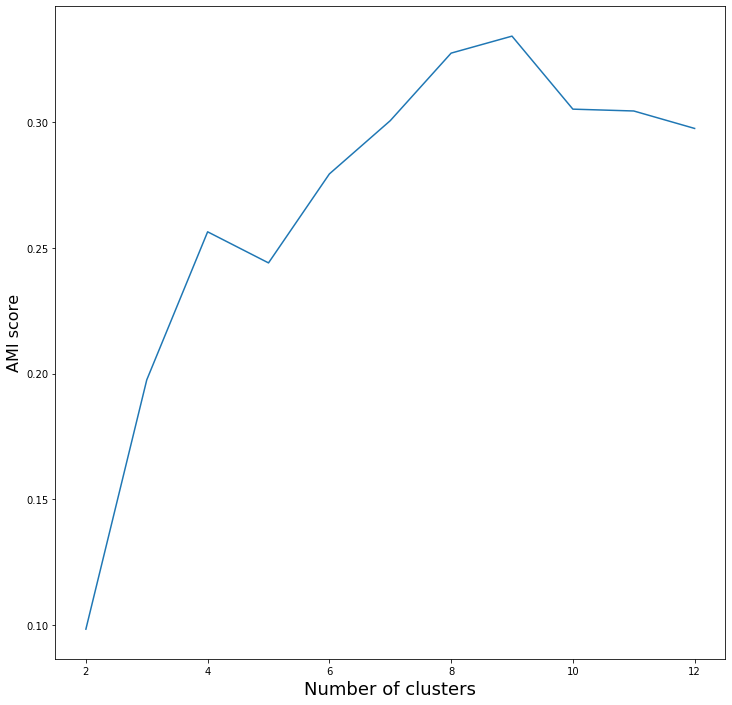
\includegraphics[width=0.9\textwidth]{ami_clusters}
\end{center}
}



\end{subquestion}

\begin{subquestion}{(3 points) Discuss any trends and interesting aspects which emerge from the plot. Does this follow from your expectations?}



\answerbox{10em}{
A trend which can be observed from the plot is how the performance keeps steadily increasing up to the point when the prediction uses 9 clusters, after which it keeps slowly decreasing. This suggests that peak performance is reached at around 9 clusters, which is very close to the true number of classes (8). Furthermore, we notice an additional local peak at 4 clusters, which corresponds to the idea that although we have 8 classes, there are 4 main topics: hardware, religion, mechanics and cryptography.
}



\end{subquestion}

\begin{subquestion}{\label{Q_CLUSTER_FOUR}(6 points) Let us investigate the case with four (4) clusters in some more detail. Using seaborn's \href{https://seaborn.pydata.org/generated/seaborn.countplot.html}{\texttt{countplot}} function, plot a bar-chart of the number of data-points with a particular class (encoded by colour) assigned to each cluster centre (encoded by position on the plot's x-axis). As part of the cluster labels, include the total number of data-points assigned to that cluster.}



\answerbox{40em}{
\begin{center}
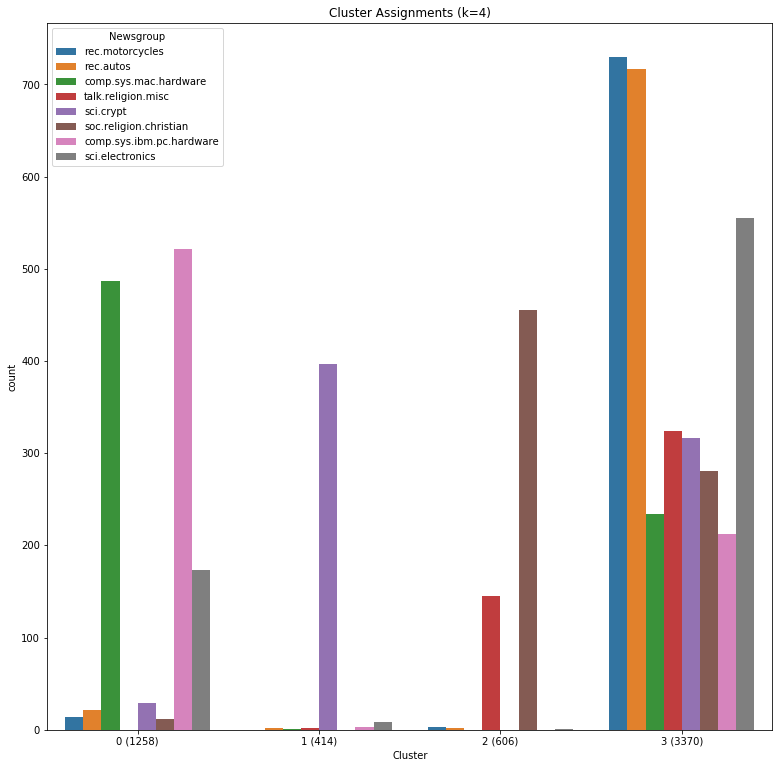
\includegraphics[width=0.9\textwidth]{cluster_assignments}
\end{center}
}



\end{subquestion}

\begin{subquestion}{(3 points) How does the clustering in Question\ref{Q_UNSUP_LEARN}:\ref{Q_CLUSTER_FOUR} align with the true class labels? Does it conform to your observations in Q 2(e)?}



\answerbox{14em}{
Clustering in Q 2(f) aligns fairly accurately with the true class labels, with the mention that Cluster 3 accumulates around 59\% of all the data-points, while Cluster 1 is left with 7\%. Cluster 0 has successfully grouped together two similar classes 'comp.sys.mac.hardware' and 'comp.sys.ibm.pc.hardware', while cluster 2 has also grouped together two similar classes:'talk.religion.misc' and 'soc.religion.christian'. Cluster 1 has isolated the independent class 'sci.crypt', and Cluster 3 has grouped together classes 'rec.motorcycles', 'rec.autos', and even 'sci.electronics'. This is in direct accordance with the observations at Q 2(e), where the AMI scores shows a general peak of performance close to 8 clusters as well as at 4 clusters.
}



\end{subquestion}



\end{question}

%============================================================================%

\begin{question}{(26 points) Logistic Regression Classification}
\label{Q_LR_NG}
\questiontext{We will now try out supervised classification on this data. We will focus on Logistic Regression and measure performance in terms of the \href{https://scikit-learn.org/stable/modules/generated/sklearn.metrics.f1_score.html}{F1} score (familiarise yourself with this score which is related to the precision and recall scores that we learnt about in class).}



\begin{subquestion}{(3 points) What is the F1-score, and why is it preferable to accuracy in our problem? How does the macro-average work to extend the score to multi-class classification?}



\answerbox{8em}{
The F1-score is the harmonic mean of recall and precision: $\frac{2 \times precision \times recall}{precision \times recall}$, where recall is $\frac{TP}{TP+FP}$ and precision is $\frac{TP}{TP+FN}$. This is preferable to accuracy because of the imbalanced class distribution. In multi-class classification, the final score (using the macro-average setting) is the unweighted mean of the F1-scores for each class. 
}



\end{subquestion}


\begin{subquestion}{(2 points) As always we start with a simple baseline classifier. Define such a classifier (indicating why you chose it) and report its performance on the \textbf{Test} set. Use the `macro' average for the \texttt{f1\_score}.} %\hint{For the baseline, the classifier should use only the target labels.}



\answerbox{8em}{
The baseline classifier for this task will generate predictions by respecting the training set’s class distribution. This is the DummyClassifier with strategy set to 'stratified', and obtains an F1-score of 0.13 on the Test set. I chose this classifier because of its simplistic approach and linear ROC curve (false positives rates plotted against true posives rates).
}



\end{subquestion}

\begin{subquestion}{(3 points) We will now train a \href{https://scikit-learn.org/stable/modules/generated/sklearn.linear_model.LogisticRegression.html}{LogisticRegression} Classifier from SKLearn. By referring to the documentation, explain how the Logistic Regression model can be applied to classify multi-class labels as in our case. \hint{Limit your explanation to methods we discussed in the lectures.}}



\answerbox{9em}{
Your Answer Here
}



\end{subquestion}

\begin{subquestion}{(4 points) Train a Logistic Regressor on the training data. Set \texttt{solver=`lbfgs'}, \texttt{multi\_class=`multinomial'} and \texttt{random\_state=0}. Use the Cross-Validation object you created and report the average validation-set F1-score as well as the standard deviation. Comment on the result.}



\answerbox{9em}{
By training a Logistic Regressor on the training data, we obtain an average F1-score of 0.67 with a fairly small standard deviation: 0.017. This translates to a major improvement over the baseline classifier because of the consistently higher F1-scores obtained (as indicated by the small standard deviation).
}



\end{subquestion}

\begin{subquestion}{\label{Q_LOG_REG_PLT}(5 points) We will now optimise the Regularisation parameter $C$ using cross-validation. Train a logistic regressor for different values of $C$: in each case, evaluate the F1 score on the training and validation portion of the fold. That is, for each value of $C$ you must provide the training set and validation-set scores per fold and then compute (and store) the average of both over all folds. Finally plot the (average) training and validation-set scores as a function of $C$. \hint{Use a logarithmic scale for $C$, spanning 19 samples between $10^{-4}$ to $10^5$.}}



\answerbox{40em}{
\begin{center}
	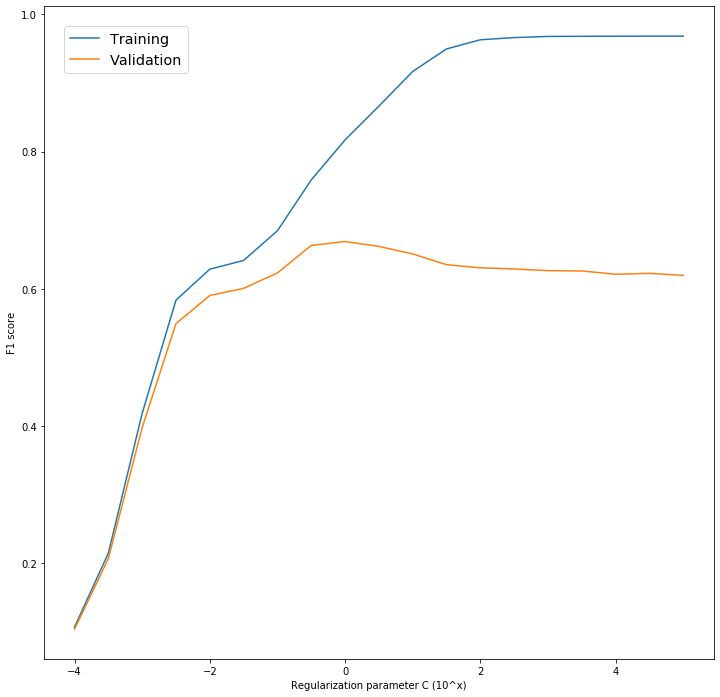
\includegraphics[width=0.9\textwidth]{regularisation_param}
\end{center}
}



\end{subquestion}

\begin{subquestion}{(7 points) What is the optimal value of $C$ (and the corresponding score)? How did you choose this value? By making reference to the effect of the regularisation parameter $C$ on the optimisation, explain what is happening in your plot from Question \ref{Q_LR_NG}:\ref{Q_LOG_REG_PLT} \hint{Refer to the documentation for $C$ in the \href{https://scikit-learn.org/stable/modules/generated/sklearn.linear_model.LogisticRegression.html}{LogisticRegression} page on SKLearn}.}



\answerbox{11em}{
The optimal value of C can be found at the point where performance on the validation set is high, but performance on the training set is low enough not to indicate overfitting. This can be observed in the plot at Q 3(e) at around x=-0.5 (corresponding to a C value of 0.32 and an F1-score of 0.66). The plot displays the evolution of the performance of classification as the penalty for increasing the magnitude of parameter values decreases (smaller values of C specify stronger regularisation). We notice how as regularisation weakens, overfitting starts to take place.
}



\end{subquestion}

\begin{subquestion}{(2 points) Finally, report the score of the best model on the test-set, after retraining on the entire training set (that is drop the folds). \hint{You may need to set \texttt{max\_iter = 200}.} Comment briefly on the result.}



\answerbox{7em}{
After retraining the Logistic Regressor on the entire training set, the F1-score of the best model (C=10\textsuperscript{-0.5}) on the test-set is 0.66. 
}



\end{subquestion}


\end{question}




%============================================================================%




%%%%%%%%%%%%%%%%%%%%%%%%%%%%%%%%%%%%%%%%%%%%%%%%%%%%%%%%%%%%%%%%%%%%%%%%%%%%%%
%============================================================================%
%%%%%%%%%%%%%%%%%%%%%%%%%%%%%%%%%%%%%%%%%%%%%%%%%%%%%%%%%%%%%%%%%%%%%%%%%%%%%%

\clearpage

\assignmentSection{Part B: Bristol Air-Quality [90 points]}




\begin{question}{\label{Q_EXPLORATORY}(30 Points) Exploratory Analysis}

\questiontext{We will begin by exploring the Dataset to familiarise ourselves with it.}



\begin{subquestion}{(6 points) Summarise the key features/observations in the data: describe the purpose of each column and report (briefly) also on the dimensionality/ranges (ballpark figures only, and how they compare across features) and number of sites, and identify anything out of the ordinary/problematic: \ie look out for missing data and negative values. Why are the latter unreasonable in such a dataset? \hint{Refer to the documentation for how to interpret the pollutant values.}}



\answerbox{13em}{
The data-set has 1306758 measurements (rows) with 7 attributes (columns) each: {\em SiteID}, {\em Loc.Lat} and {\em Loc.Long} identify the location, {\em Date Time} the moment of measurement and {\em $NO_{x}$}, {\em $NO_{2}$} and {\em NO} are obtained from chemiluminescent analysers (API T200) in $\frac{\mu g}{m^{3}}$. {\em $NO_{x}$} has a higher range (up to 2164) when compared to {\em $NO_{2}$} (576) and {\em NO} (1231). There are 18 sites, numbered 0 to 17. Missing data and negative values occur quite often. The latter are unreasonable here because they defy the logic of the data: pollutant values as measured by the API T200 analysers should never be negative (unless because of calibration errors or the corruption of the Auto Zero  filter), as should any of the other columns.
}



\end{subquestion}

\begin{subquestion}{(6 points) Repeat the same analysis but this time on a per-site basis. Provide a table with the number of samples and percentage of problematic samples (negative and missing) in each site. To report numbers, count a row which has at least one missing entry
as having missing data, and similarly for negative entries. \hint{Pandas has a handy method, \texttt{to\_latex()}, for generating a latex table from a dataframe.}}



\answerbox{17em}{
\scalebox{0.65} {
	\begin{tabular}{rrr}
		 SiteID &   \# Samples &  \% Problematic samples \\
		 \midrule    0.0 &    6446.0 & 1.613404 \\
		     1.0 &  163111.0 &  6.290195 \\
		     2.0 &   62990.0 &  4.353072 \\
		     3.0 &   25464.0 &  78.110273 \\
		     4.0 &   74787.0 &  2.072553 \\
		     5.0 &  113952.0 &  8.828279 \\
		     6.0 &  142141.0 &  7.446831 \\
		     7.0 &  115162.0 &  4.472830 \\
		     8.0 &   43824.0 &  21.056955 \\
		     9.0 &   22071.0 &  5.301074 \\
		    10.0 &   96407.0 &  3.594137 \\
		    11.0 &   20693.0 &  1.981346 \\
		    12.0 &   45240.0 &  17.484527 \\
		    13.0 &   12423.0 &  51.477099 \\
		    14.0 &  113951.0 &  10.531720 \\
		    15.0 &    2712.0 &  100.000000 \\
		    16.0 &  154331.0 &  6.544375 \\
		    17.0 &   91053.0 &  6.273269 \\
	\end{tabular}
}
}



\end{subquestion}

\begin{subquestion}{(4 points) Briefly summarise how the sites compare in terms of number of samples and amount of problematic samples.}



\answerbox{11em}{
Sites are unevenly distributed in terms of number of samples: the mean is of 72598 samples, but the standard deviation is very high (53066). This translates to a high variability in the number of samples among sites e.g. sites 0 and 15 have 6446 and 2712 samples, while sites 1 and 16 have 163111 and 154331 samples. In terms of problematic samples, each site has, on average, around 5\% problematic samples, but there are a few exceptions: most notably, site 8 has 21\%, site 13 has 51\%, site 3 has 78\% and site 15 has 100\% (every entry is corrupted).
}



\end{subquestion}

\begin{subquestion}{(3 points) Given that the columns are all oxides of nitrogen and hence we expect them to be related, we will now look at correlations in our data. This will also be useful in determining how well we can predict any one of the readings from the other two. Remove the data from sites 3 and 15 and compute the \textbf{Pearson} correlation coefficient between each of the three pollutant columns on the remaining data. Visualise the coefficients between each pair of columns in a table.}



\answerbox{10em}{
\scalebox{1.3} {
\begin{tabular}{lrrr}
	{} &       NOx &       NO2 &        NO \\
	\midrule NOx &  1.000000 &  0.878016 &  0.988019 \\
	NO2 &  0.878016 &  1.000000 &  0.807853 \\
	NO  &  0.988019 &  0.807853 &  1.000000 \\
\end{tabular}
}
}



\end{subquestion}

\begin{subquestion}{(2 points) Comment on the level of correlation between each pair of pollutants.}



\answerbox{7em}{
{\em $NO_{x}$} and {\em NO} have the highest correlation (0.99), followed closely by {\em $NO_{x}$} and {\em $NO_{2}$} at 0.88, and {\em NO} and {\em $NO_{2}$} at 0.8. We notice that all pairs of pollutants are generally very highly correlated.
}



\end{subquestion}



\begin{subquestion}{\label{CORRELATIONS}(5 points) For each of the three pollutants, compute the Pearson correlation between sites. \hint{You will need to remove the `Date Time' column and then group by the first level of the columns.} Then plot these as three heatmaps: show the values within the figures. \hint{Use the method \texttt{plot\_matrix()} from \texttt{mpctools.extensions.mplext}.}}



\answerbox{40em}{
\begin{center}
	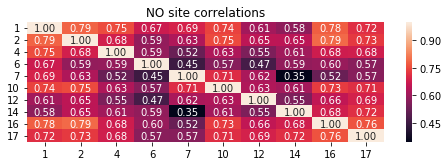
\includegraphics[width=0.9\textwidth]{no}
\end{center}
\begin{center}
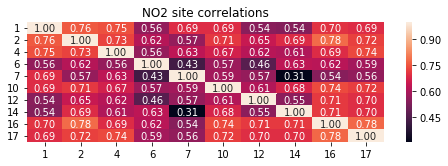
\includegraphics[width=0.9\textwidth]{no2}
\end{center}
\begin{center}
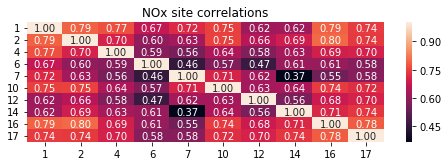
\includegraphics[width=0.9\textwidth]{nox}
\end{center}
}



\end{subquestion}

\begin{subquestion}{(4 points) Comment briefly on your observations from Question \ref{Q_EXPLORATORY}:\ref{CORRELATIONS}: start by summarising the results from the NO gas and then comment on whether the same is observed in the other gases or if there is something different.}



\answerbox{12em}{
The NO gas indicates correlations of over 0.5 overall, with two exceptions being between sites 14 and 7 (0.35), and between sites 7 and 6 (0.45) and 12 and 6 (0.47). The same exceptions are found in the NO2 and NOx site correlation heatmaps.
}



\end{subquestion}

\end{question}


%============================================================================%

\begin{question}{(19 Points) Principal Component Analysis}

\questiontext{One aspect which we have not yet explored is the temporal nature of the data. That is, we need to keep in mind that the readings have a temporal aspect to them which can provide some interesting insight. We will explore this next.}



\begin{subquestion}{(1 point) Plot the first 5 lines of data (plot each row as a single line-plot).}



\answerbox{40em}{
\begin{center}
	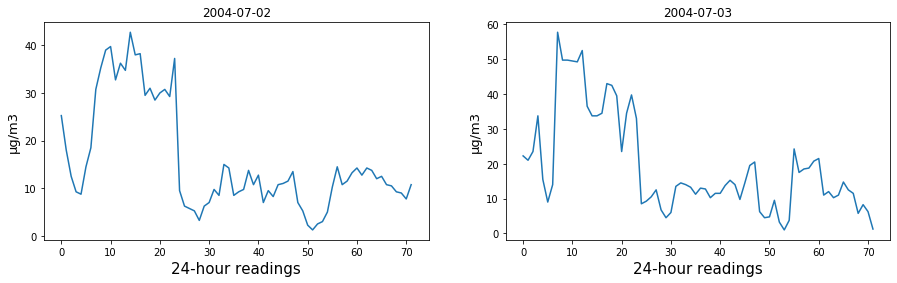
\includegraphics[width=0.9\textwidth]{lines12}
\end{center}
\begin{center}
	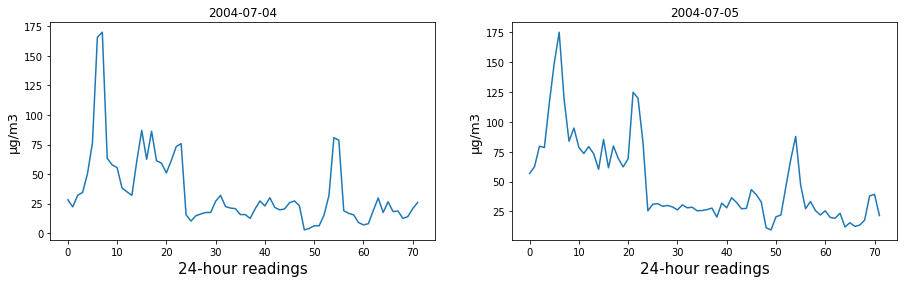
\includegraphics[width=0.9\textwidth]{lines34}
\end{center}
\begin{center}
\scalebox{0.7} {
	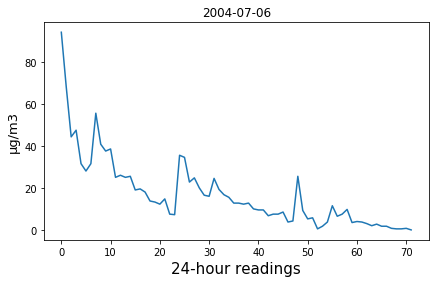
\includegraphics[width=0.9\textwidth]{line5}
}
\end{center}
}



\end{subquestion}



\begin{subquestion}{(5 points) We will focus first on data solely from Site 1. Extract the data from this site, and run PCA with the number of components set to 72 for now. Set the \texttt{random\_state=0}. On a single graph plot: (i) the percentage of the variance explained by each principal component (as a bar-chart), (ii) the cumulative variance (line-plot) explained by the first $n$ components: (\hint{you should use \href{https://matplotlib.org/3.1.1/api/_as_gen/matplotlib.axes.Axes.twinx.html}{\texttt{twinx()}} to make the plot fit}), \textsl{and}, (iii) mark the point at which the number of components collectively explain at least 95\% of the variance (using a vertical line). \hint{Number components starting from 1.}}



\answerbox{40em}{
Your Image Here
}



\end{subquestion}

\begin{subquestion}{(2 points) Interpret and summarise the above plot.}



\answerbox{9em}{
Your Answer Here
}



\end{subquestion}


\begin{subquestion}{(5 points) Generate three figures, one for the mean and one for each of the first 2 principal components: in each, plot the mean/component as three lines, one for each pollutant throught one day cycle. \hint{You will need to reshape the components appropriately.}}



\answerbox{50em}{
Your Image Here
}



\end{subquestion}

\begin{subquestion}{(6 points) Focusing on the mean and first principal component, are there any significant patterns which emerge throughout the day? \hint{Think about car usage throughout the day.} What is different when interpreting the mean versus the first component? \hint{Do peaks signify the same thing in both cases?} Looking at the principal components only, are there any significant differences between the pollutants? Why could this be happening? \hint{You can refer to one of the limitations of PCA.}}



\answerbox{16em}{
Your Answer Here
}



\end{subquestion}

\end{question}

%============================================================================%


\begin{question}{\label{Q_LR_BA}(41 points) Regression}


\questiontext{Given our understanding of the correlation between signals and sites, we will now attempt to predict the NOx level for Site 17 given the value at the other sites. We will evaluate our models using the Root Mean Squared Error (RMSE) \ie the square root of the \href{https://scikit-learn.org/stable/modules/generated/sklearn.metrics.mean_squared_error.html}{mean\_squared\_error} score by sklearn.}



\begin{subquestion}{(2 points) First things first: since we are dealing with a supervised task, we will need to split our data into a training and testing set. Furthermore, since some of our regressors will involve hyper-parameter tuning, we will also need a validation set. Use the \texttt{multi\_way\_split()} method from \texttt{mpctools.extensions.skext} to split the data into a Training (60\%), Validation (15\%) and Testing (25\%) set: use the \href{https://scikit-learn.org/stable/modules/generated/sklearn.model_selection.ShuffleSplit.html}{ShuffleSplit} object from sklearn for the \texttt{splitter}. Set the random state to 0. \hint{The method gives you the indices of the split for each set, which can then be applied to multiple matrices.} Report the sizes of each dataset.}



\answerbox{4em}{
Your Answer Here
}



\end{subquestion}

\begin{subquestion}{(4 points) Let us start with a baseline. By using only the $y$-values, what baseline regressor can you define (indicate what it does)? Implement it and report the RMSE on the training and validation sets. Interpret this relative to the statistics of the data.}



\answerbox{8em}{
Your Answer Here
}



\end{subquestion}

\begin{subquestion}{(3 points) Let us now try a more interesting algorithm: specifically, we will start with \href{https://scikit-learn.org/stable/modules/generated/sklearn.linear_model.LinearRegression.html}{LinearRegression}. Train the regressor on the training data and report the RMSE on the training and validation set, and comment on the relative performance to the baseline.}



\answerbox{7em}{
Your Answer Here
}



\end{subquestion}



\begin{subquestion}{(5 points) We want to explore further what the model is learning. Explain why in Linear Regression, we cannot just blindly use the weights of the regression coefficients to evaluate the relative importance of each feature, but rather we have to normalise the features. By referring to the documentation for the \href{http://scikit-learn.org/stable/modules/generated/sklearn.linear_model.LinearRegression.html}{LinearRegression} implementation in SKLearn, explain what the normalisation does and how it helps in comparing features. Will this affect the performance of the Linear Regressor?}



\answerbox{10em}{
Your Answer Here
}



\end{subquestion}

\begin{subquestion}{(5 points) Retrain the regressor, setting \texttt{normalize=True} and report (in a table) the ratio of the relative importance of each feature. Which is the most/least important site? How do they compare with the correlation coefficients for Site 17 as computed in Question \ref{Q_EXPLORATORY}:\ref{CORRELATIONS}, and why do you think that is?}



\answerbox{15em}{
Your Answer Here
}



\end{subquestion}

\begin{subquestion}{(5 points) It might be that with non-linear models, we may get better performance. Let us try to use \href{https://scikit-learn.org/stable/modules/generated/sklearn.neighbors.KNeighborsRegressor.html}{K-Nearest-Neighbours}. Train a KNN regressor with default parameters on the training set and report performance on the training and validation set. \hint{it might be beneficial to set \texttt{n\_jobs=-1} to improve performance.} How does it compare with Linear Regression in terms of performance on both sets? What is a limitation of the KNN algorithm for our dataset?}



\answerbox{8em}{
Your Answer Here
}



\end{subquestion}

\begin{subquestion}{(4 points) The KNN regression allows setting a number of hyper-parameters. We will optimise only one: the number of neighbours to use. By using the validation set, find the optimal value for the \texttt{n\_neighbours} parameter out of the values [2, 4, 8, 16, 32]. Plot the training/validation RMSE and indicate (for example with a line) the best value for \texttt{n\_neighbours}.}



\answerbox{40em}{
Your Image Here
}



\end{subquestion}

\begin{subquestion}{(1 points) What is the best-case RMSE performance on the validation set for KNN?}



\answerbox{6em}{
Your Answer Here
}



\end{subquestion}

\begin{subquestion}{(4 points) Let us try one last regression algorithm: we will now use \href{https://scikit-learn.org/stable/modules/generated/sklearn.tree.DecisionTreeRegressor.html}{DecisionTreeRegressor}. Again, the algorithm contains a number of hyper-parameters, and we will optimise the depth of the tree. Train a series of Decision Tree Regressors, optimising (over the validation set) the \texttt{max\_depth} over the values [2, 4, 8, 16, 32, 64]. Set \texttt{random\_state=0}. Plot the training/validation RMSE and indicate (as before) the best value for \texttt{max\_depth}.}



\answerbox{40em}{
Your Image Here
}



\end{subquestion}

\begin{subquestion}{(3 points) What is the best-case RMSE performance on the validation set? What do you notice from the plot about the performance of the Decision Tree Regressor?}



\answerbox{6em}{
Your Answer Here
}



\end{subquestion}

\begin{subquestion}{(5 points) To conclude let us now compare all the models on the testing set. Combine the training and validation sets and retrain the model from each family on it: in cases where we optimised hyper-parameters, set this to the best-case value. Report the testing-set performance of each model in a table \hint{You should have 4 values}.}



\answerbox{6em}{
Your Answer Here
}



\end{subquestion}

\end{question}

%============================================================================


\end{document}
